\documentclass[a4paper,11pt]{article}
\usepackage[T1]{fontenc}
\usepackage[latin2]{inputenc}
\usepackage{amsfonts}
\usepackage{amssymb}
\usepackage{amsthm}
\usepackage{amsmath} 
\usepackage[polish]{babel}
\usepackage{graphicx}
\usepackage{times}
\usepackage{anysize}
\usepackage{color}

\marginsize{1.5cm}{1.5cm}{1.5cm}{1.5cm}
\sloppy 

\def\etya{$\int_a^b f(x)dx \approx h \sum_{i=1}^n f(x_i)$}
\def\etyb{$y = f(x)$}
\def\etyc{$x_0 = a$}
\def\etyd{$x_i$}
\def\etye{$x_n = b$}
\def\etyf{$h$}

\begin{document}

\section{Wersja z wzorami}

Wzory umieszczamy bezpo�rednio w xfigu.

\begin{figure}[!htb]
\centerline{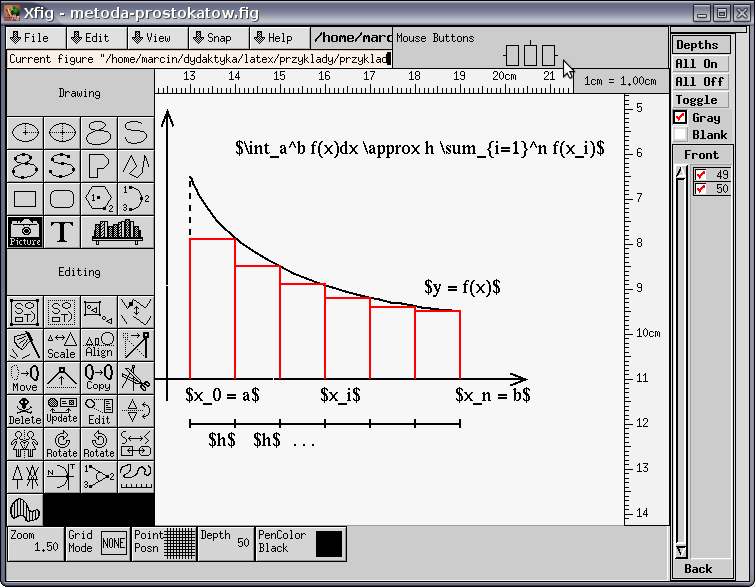
\includegraphics[scale=0.5]{xfig1}}
\caption{Xfig - zrzut ekranu 1}
\label{fig:xfig1}
\end{figure}

Etykiety tekstowe, kt�re maj� by� interpretowane jako wzory matematyczne musz� mie� ustawion� flag�: \textit{Text flags} $\to$ \textit{Special flag} $\to$ \textit{Special}. Dla zwyk�ego tekstu ta flaga ma warto�� \textit{normal}. 

\begin{figure}[!htb]
\centerline{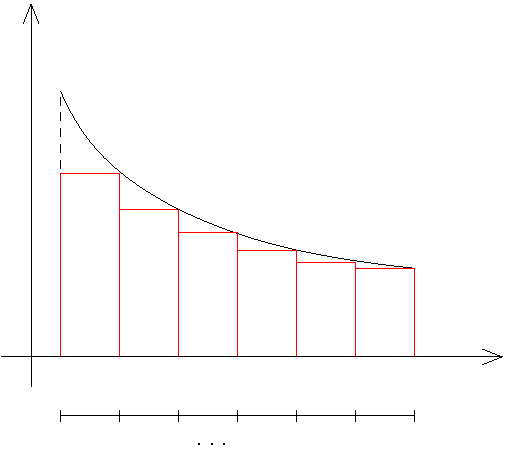
\includegraphics[scale=1]{metoda-prostokatow}}
\caption{Wyeksportowany plik pdf (w. 1)}
\label{fig:xfig1pdf}
\end{figure}

\begin{figure}[!htb]
\centerline{\resizebox{!}{7.5cm}{\input{metoda-prostokatow.pdf_t}}}
\caption{Rysunek z wzorami (w. 1)}
\label{fig:xfig1complete}
\end{figure}


\section{Wersja z etykietami}

\begin{figure}[!htb]
\centerline{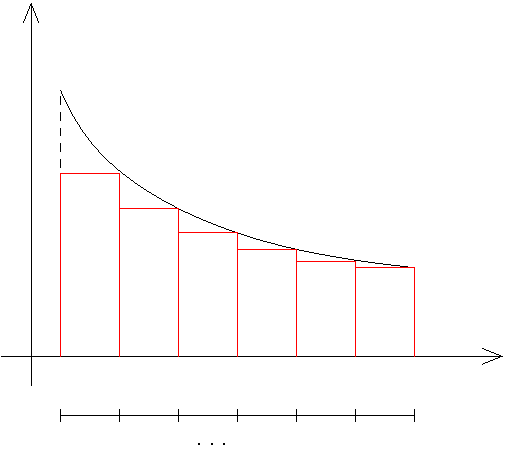
\includegraphics[scale=1]{metoda-prostokatow2}}
\caption{Wyeksportowany plik pdf (w. 2)}
\label{fig:xfig2pdf}
\end{figure}

\begin{figure}[!htb]
\centerline{\resizebox{!}{7.5cm}{\input{metoda-prostokatow2.pdf_t}}}
\caption{Rysunek z wzorami (w. 2)}
\label{fig:xfig2complete}
\end{figure}


\end{document}

